%!TEX program = pdflatex
\documentclass[runningheads]{llncs}
%
\usepackage{booktabs}
\usepackage{multirow}
\usepackage[T1]{fontenc}
\usepackage{lmodern}

% T1 fonts will be used to generate the final print and online PDFs,
% so please use T1 fonts in your manuscript whenever possible.
% Other font encodings may result in incorrect characters.
%
\usepackage{graphicx,verbatim}
% Used for displaying a sample figure. If possible, figure files should
% be included in EPS format.
%
% If you use the hyperref package, please uncomment the following two lines
% to display URLs in blue roman font according to Springer's eBook style:
%\usepackage{color}
%\renewcommand\UrlFont{\color{blue}\rmfamily}
%\urlstyle{rm}
%
\usepackage[pagebackref=true,breaklinks=true,colorlinks,bookmarks=false]{hyperref}
\usepackage{xurl}
\begin{document}
%
\title{User-Friendly AI Software for Automated Quantitative CMR Reporting on Low-Cost, Energy-Efficient Devices}
\titlerunning{Accessible AI for Automated CMR Reporting}
%\titlerunning{Abbreviated paper title}
% If the paper title is too long for the running head, you can set
% an abbreviated paper title here
%
\author{Minh Nhat Trinh\inst{1} \and
Teresa M Correia\inst{1,2}
} 
%
\authorrunning{Minh Nhat Trinh and Teresa M Correia}
% First names are abbreviated in the running head.
% If there are more than two authors, 'et al.' is used.
%
\institute{Quantitative Bio-imaging Lab, Centro de Ciências do Mar (CCMAR/CIMAR-LA), Campus de Gambelas, Universidade do Algarve, Faro, Portugal
\and
 School of Biomedical Engineering and Imaging Sciences, King's College London, London, United Kingdom \\
\email{tmcorreia@ualg.pt}}


% \author{Anonymized Authors}  %% Added for anonymized MICCAI submission
% \authorrunning{Anonymized Author et al.}
% \institute{Anonymized Affiliations \\
%     \email{email@anonymized.com}}
  
\maketitle              % typeset the header of the contribution
%
\begin{abstract}

Cardiac magnetic resonance (CMR) is the reference standard for assessing cardiac function and viability, yet its clinical adoption remains limited in many resource-constrained settings due to shortages of specialized staff and the computational requirements of existing AI solutions. Here, we introduce \textit{Myopari}, an open-source Napari plugin for automated quantitative CMR analysis on low-cost, energy-efficient edge devices. The framework integrates a lightweight FC-DenseNet segmentation model with automated biomarker extraction, three-dimensional visualization, and structured patient report generation within an intuitive graphical user interface. The proposed model contains only 1.4 million parameters ($\sim$5 MB) while maintaining robust segmentation performance on the ACDC and EMIDEC datasets. Deployment on the NVIDIA Jetson Orin Nano and Raspberry Pi 5 achieved inference times of approximately 2.2 s and 10.6 s per patient, respectively, with no statistically significant differences in segmentation performance compared with a GPU workstation ($p>0.05$). \textit{Myopari} enables fully automated analysis through a single-click workflow without requiring dedicated GPU hardware or programming expertise. By combining accurate AI-assisted CMR analysis with affordable hardware and user-friendly software, \textit{Myopari} provides a practical and sustainable solution for expanding access to advanced cardiac imaging in low- and middle-income countries and other resource-constrained healthcare settings. The software and source code are publicly available at \href{https://github.com/QBioImaging/myopari}{github.com/QBioImaging/myopari}. 
\keywords{Cardiac MRI \and Edge AI \and  Automated Quantitative Reporting \and Image Segmentation}
\end{abstract}

\section{Introduction}

Cardiovascular disease remains one of the leading causes of mortality worldwide, with the burden disproportionately affecting low- and middle-income countries (LMICs), where access to specialized cardiac imaging expertise is often limited \cite{chong2025global}. Cardiac magnetic resonance (CMR) is the gold standard for evaluating cardiac function and viability \cite{kawel2020reference}; however, routine CMR analysis requires labor-intensive segmentation and quantitative measurements that depend on experienced readers and substantial reporting time \cite{chen2020deep}, hindering its adoption in under-resourced settings where magnetic resonance imaging (MRI) is available.  

Recently, deep learning methods have achieved near-human performance in automated CMR segmentation and quantitative analysis \cite{chen2020deep,bai2018automated,U-Net,fan2023vit}. Nevertheless, most existing solutions are designed for GPU-equipped workstations and require complex software environments or expensive commercial licenses, limiting their accessibility in resource-constrained settings (RCS). Consequently, despite remarkable algorithmic advances, practical deployment of AI-assisted CMR analysis remains a challenge in many healthcare systems.

Recent progress in edge AI provides an opportunity to address these limitations. Low-cost devices such as the Raspberry Pi~5 \cite{raspberry} and NVIDIA Jetson Nano \cite{jetsonnano} can efficiently execute lightweight deep learning models while consuming significantly less power than conventional GPU workstations. Moreover, Napari \cite{napari}, an open-source Python-based biomedical image viewer with a flexible plugin architecture, offers an intuitive platform for integrating AI models into clinical workflows without requiring programming expertise.

In this work, we present \textit{Myopari}, an open-source Napari plugin for automated quantitative CMR analysis on low-cost edge devices. The proposed framework integrates a lightweight deep learning model for CMR segmentation with automated biomarker extraction, three-dimensional (3D) visualization, and structured patient report generation within a user-friendly GUI. Unlike existing approaches that primarily emphasize segmentation accuracy or inference optimization, \textit{Myopari} combines accurate AI-assisted CMR analysis, resource-efficient deployment, and one-click clinical reporting into a single deployable application. By lowering computational, financial, and technical barriers, \textit{Myopari} aims to improve access to advanced cardiac imaging workflows in resource-constrained healthcare settings.

\section{Methodology}
The proposed framework consists of three components: (1) a lightweight deep learning model for automated CMR segmentation, (2) post-training quantization and deployment on low-cost edge hardware for efficient inference, and (3) an integrated Napari plugin for fast 3D visualization and automated quantitative report generation. An overview of the framework is shown in Fig.~\ref{fig:framework}.
\begin{figure}[!ht]
    \centering
    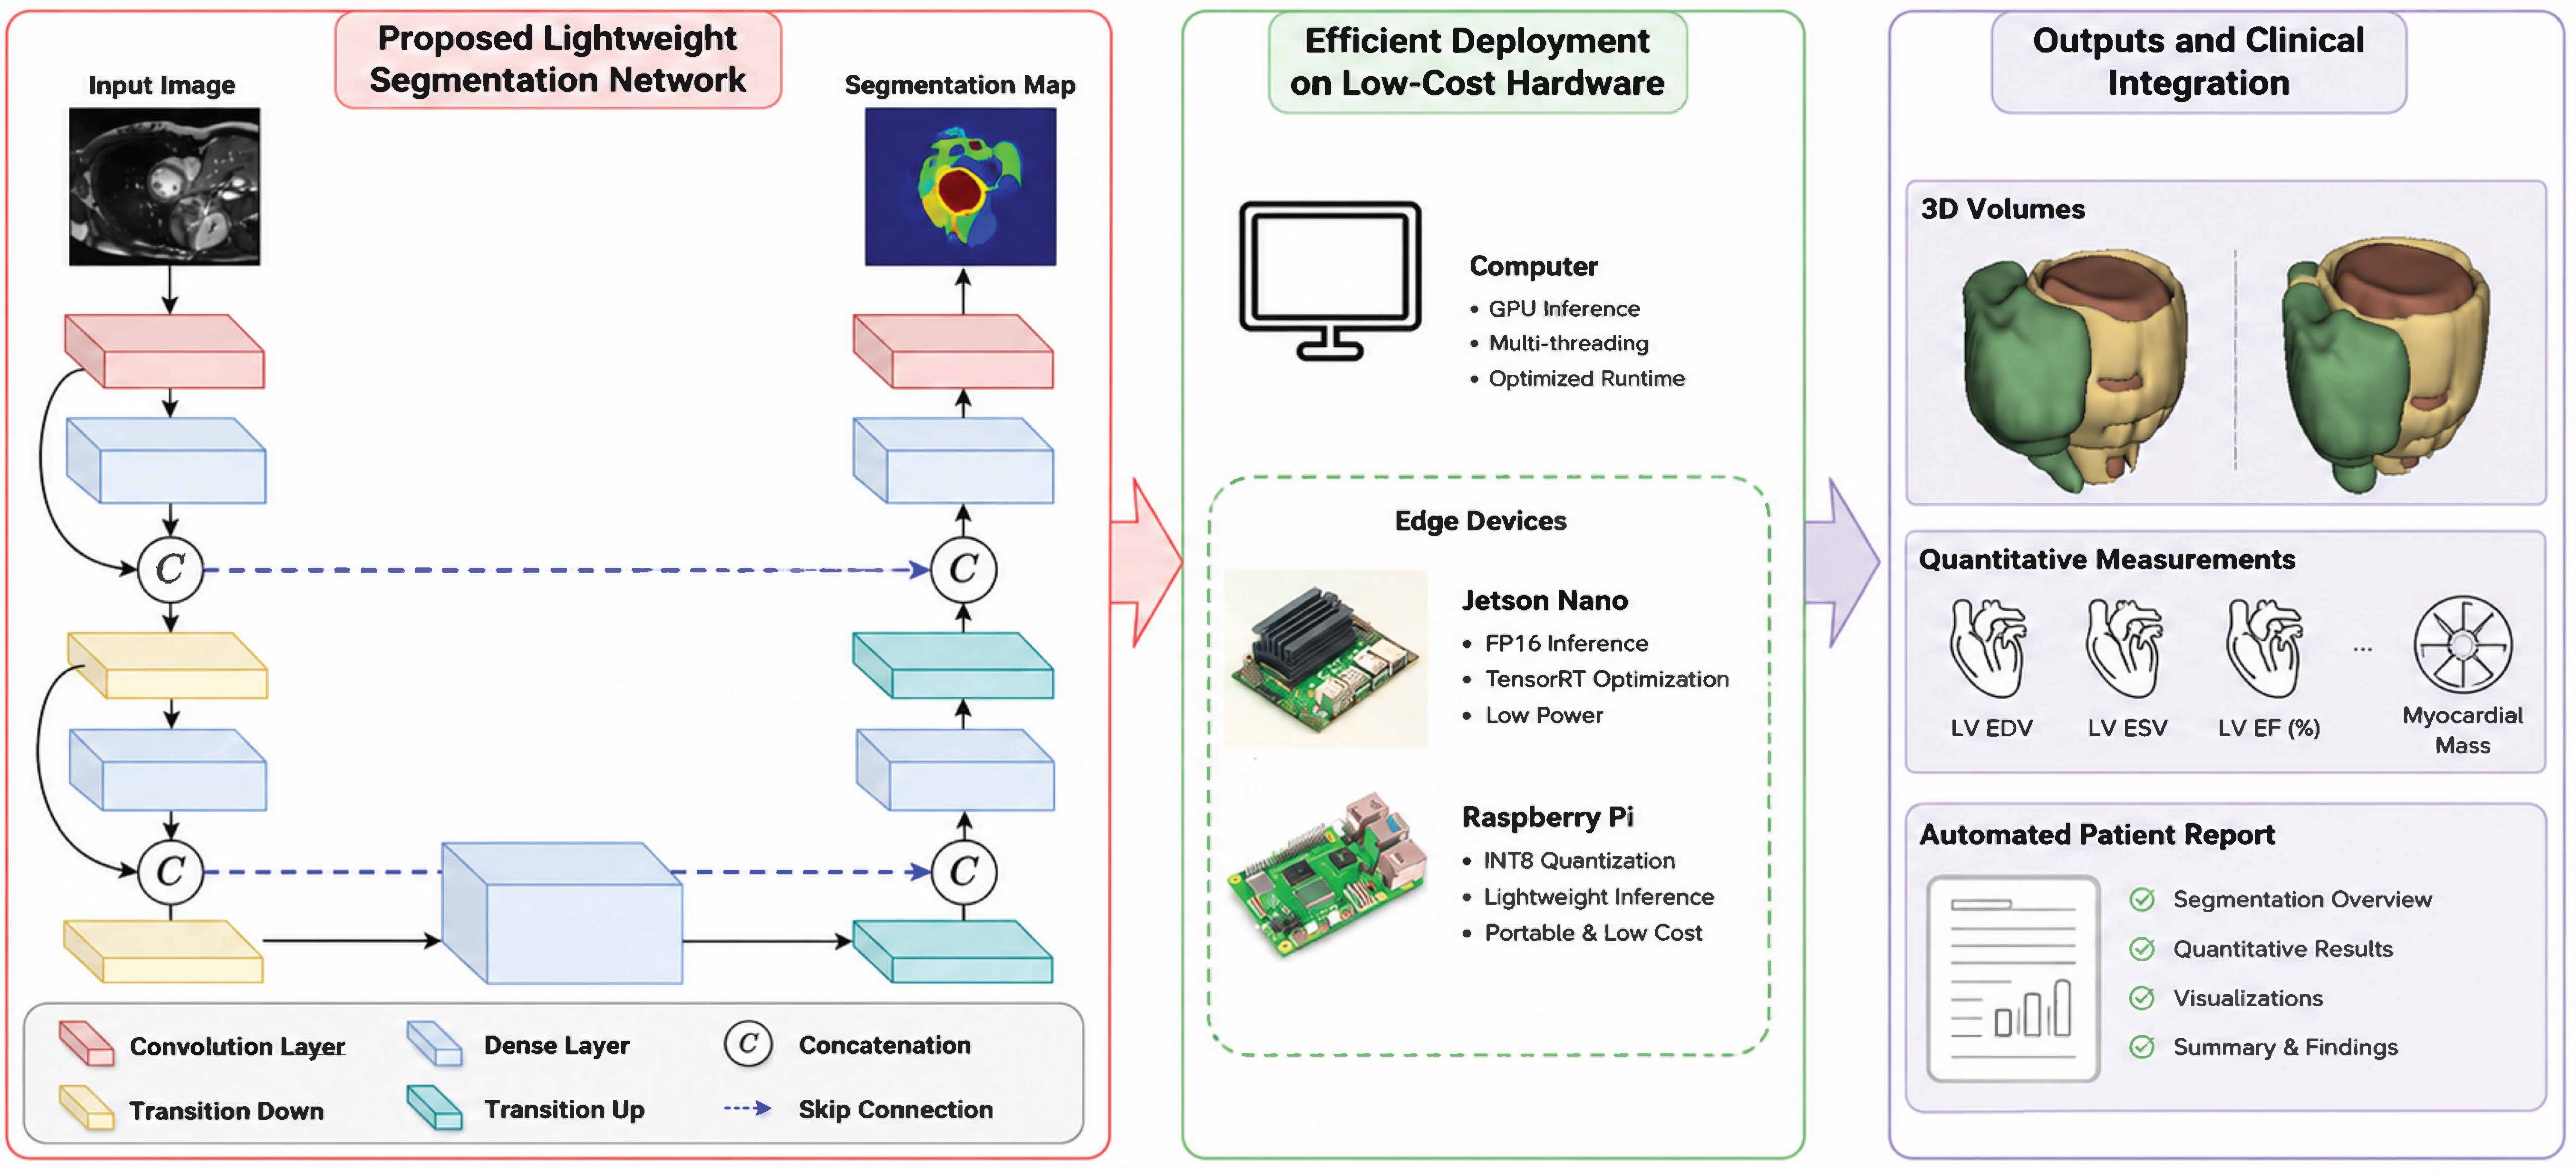
\includegraphics[width=\linewidth]{images/model.pdf}
    \caption{Proposed AI-powered framework for automated CMR analysis and quantitative reporting on low-cost, energy-efficient hardware.}
    \label{fig:framework}
\end{figure}
\subsection{Lightweight CMR Segmentation Network}

To enable deployment on resource-constrained hardware, we adopted a compact fully convolutional DenseNet (FC-DenseNet) architecture based on the U-Net encoder--decoder framework \cite{tiramisu}. The network contains approximately 1.4 million parameters, occupies only $\sim$5 MB of storage, and requires 12.01 GFLOPs per inference, making it suitable for embedded devices with limited memory and computational resources.

Model compactness was achieved using a shallow FC-DenseNet configuration with five encoder and decoder dense blocks $(4,4,4,4,4)$, a growth rate of 12, and 48 feature maps in the initial convolution layer. Dense skip connections preserve feature reuse throughout the network, while substantially reducing the number of parameters compared to conventional U-Net architectures. This design provides an effective balance between segmentation accuracy and computational efficiency.

\subsection{Datasets and Training Strategy}
The proposed framework was evaluated on two publicly available benchmark datasets: \textbf{EMIDEC} \cite{emidec} consists of 100 late gadolinium enhancement (LGE) CMR studies (33 normal and 67 pathological), each containing 5--10 short-axis slices acquired on 1.5T and 3.0T Siemens scanners. Images have an in-plane pixel spacing ranging from $1.25 \times 1.25$ mm$^2$ to $2.0 \times 2.0$ mm$^2$ and a slice thickness of 8 mm. The dataset was divided into 70 training, 10 validation, and 20 testing cases. Target structures include the left ventricle (LV), myocardium (Myo), microvascular obstruction (MVO)/no-reflow and myocardial infarction (MI) regions for viability assessment. \textbf{ACDC 2017} \cite{acdc} contains 150 cine CMR cases acquired on 1.5T and 3.0T Siemens scanners, each with 28--40 slices, in-plane pixel spacing of 1.37--1.68 mm, and a slice thickness of 5--8 mm. Following the official split, 80, 20, and 50 cases were used for training, validation, and testing, respectively. Annotations included the LV, right ventricle (RV), and Myo at both end-diastolic (ED) and end-systolic (ES) phases.

Training was performed on an NVIDIA GeForce RTX 4070 SUPER GPU (12 GB) using mixed-precision (FP16/FP32) computation. Images were cropped and resized to $256 \times 256$ pixels before training. The network was optimized with the NAdam optimizer \cite{nadam} (learning rate $10^{-3}$) for approximately 500 epochs, requiring about 5 hours. To improve segmentation under class imbalance and enhance boundary delineation, the Focal Active Contour Loss \cite{focal_active_loss}, combining focal weighting with active contour regularization, was employed. After training, the model was converted to the ONNX format for efficient inference and deployment on low-cost edge devices, including the NVIDIA Jetson Orin Nano Developer Kit and Raspberry Pi 5. Model performance was evaluated on ACDC and EMIDEC by comparing the predicted segmentations with the reference annotations using the Dice similarity coefficient (Dice), Hausdorff distance (HD), and volume difference. For EMIDEC, scar burden (\% infarcted myocardium) was also assessed.
\subsection{\textit{Myopari}: User-Friendly AI-based Analysis Software}
To facilitate deployment in clinical and resource-constrained settings, we developed \textit{Myopari}, a Napari plugin that integrates lightweight CMR segmentation models into an intuitive GUI (Fig.~\ref{fig:myopari}).
\begin{figure}[!ht]
    \centering
    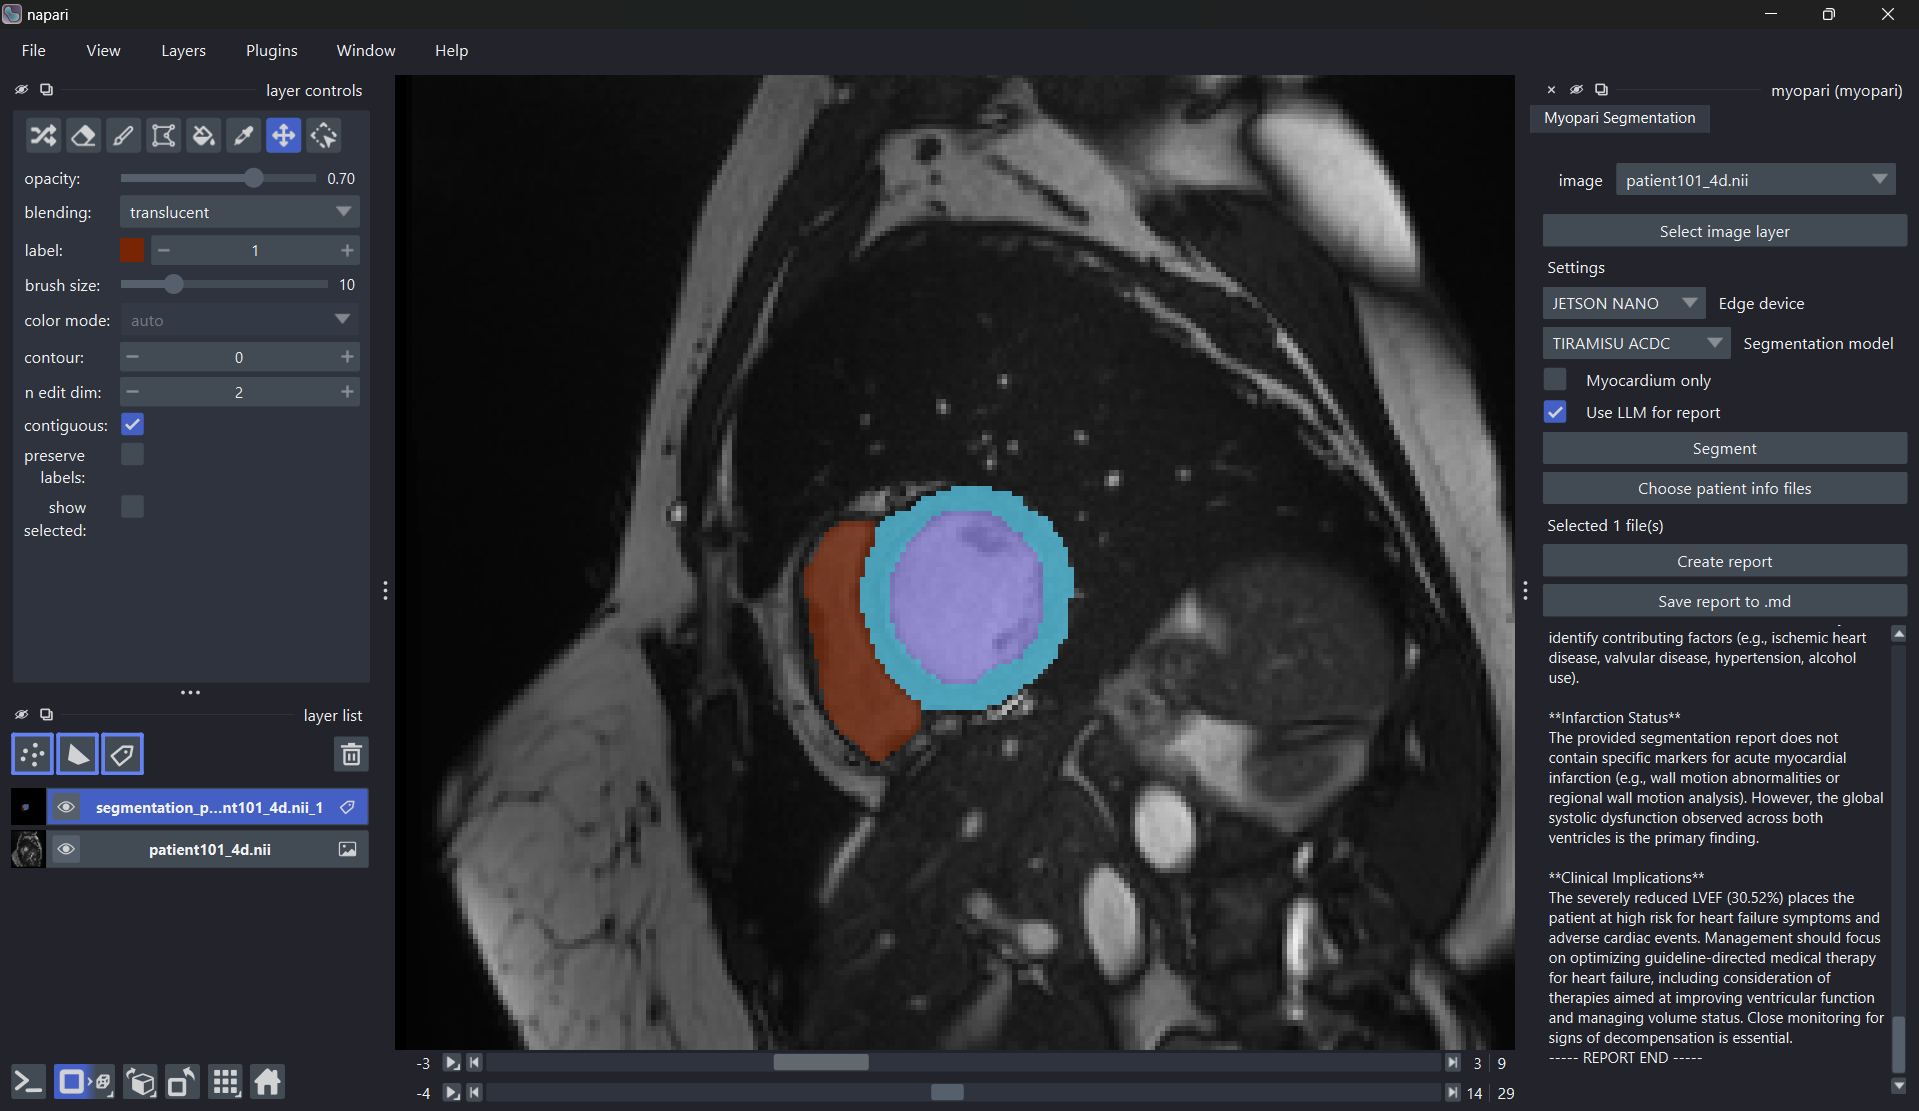
\includegraphics[width=0.9\linewidth]{images/myopari.png}
    \caption{\textit{Myopari} Napari plugin for automated CMR analysis. This simple workflow enables automated segmentation, biomarker extraction, 3D rendering, and structured reporting. Users only need to select the hardware and AI model; the plugin then executes the full analysis pipeline with one click.}
    \label{fig:myopari}
\end{figure}
Unlike command-line research software, \textit{Myopari} enables fully automated CMR analysis through a simple point-and-click workflow. First, users select the target hardware platform, either NVIDIA Jetson Nano (hybrid GPU--CPU inference) or Raspberry Pi 5 (CPU-only inference). Then, users choose the appropriate segmentation model for the target dataset (e.g., cine or LGE CMR) and may optionally enable myocardium-only segmentation and automatic report generation. Finally, the entire analysis pipeline is executed by pressing a single \textit{Segment} button. \textit{Myopari} automatically performs image segmentation, computes quantitative cardiac biomarkers, generates 3D visualizations, and produces a structured patient report. This streamlined workflow lowers the technical barrier to AI-assisted CMR analysis, making advanced CMR analysis accessible on affordable, low-energy computing platforms. To promote reproducibility and community development, \textit{Myopari} is released as open source and is available at \href{https://github.com/QBioImaging/myopari}{github.com/QBioImaging/myopari}.
\begin{figure}[!ht]
    \centering
    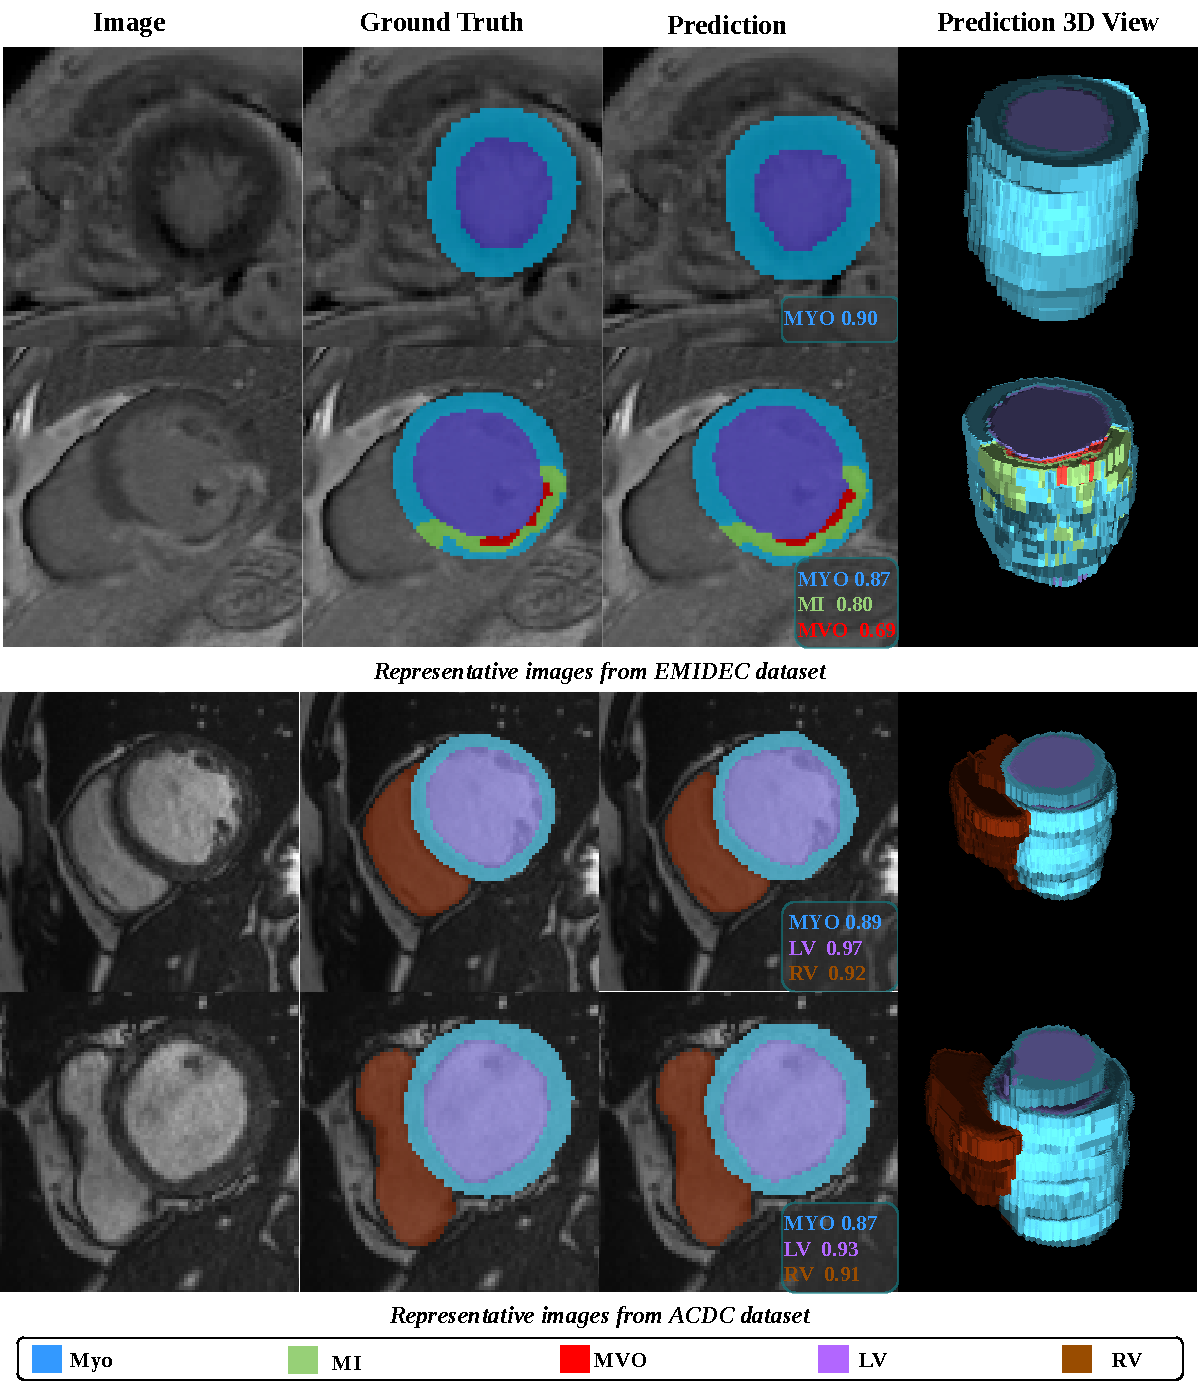
\includegraphics[width=0.8\linewidth]{images/samples.pdf}
    \caption{Representative cases from the EMIDEC and ACDC datasets. From left to right: LGE image, ground truth segmentation, model prediction, and 3D rendering in Napari. Segmentation labels are color-coded as follows: left ventricle (LV), myocardium (Myo), right ventricle (RV), myocardial infarction (MI), and microvascular obstruction (MVO, also referred to as no-reflow).}
    \label{fig:sample}
\end{figure}
\section{Results}
Figures~\ref{fig:sample} and \ref{fig:metrics} show that the proposed model produces accurate segmentations across both datasets. 
Predicted contours closely match the reference annotations, with consistently high Dice scores and low HD and volume differences. Although Dice is sensitive to small boundary errors in tiny pathological regions such as MVO and small infarcts, scar burden estimation remained highly consistent with the ground truth, with no statistically significant difference ($p=0.24$, Wilcoxon signed-rank test).
\begin{figure}[!ht]
    \centering
    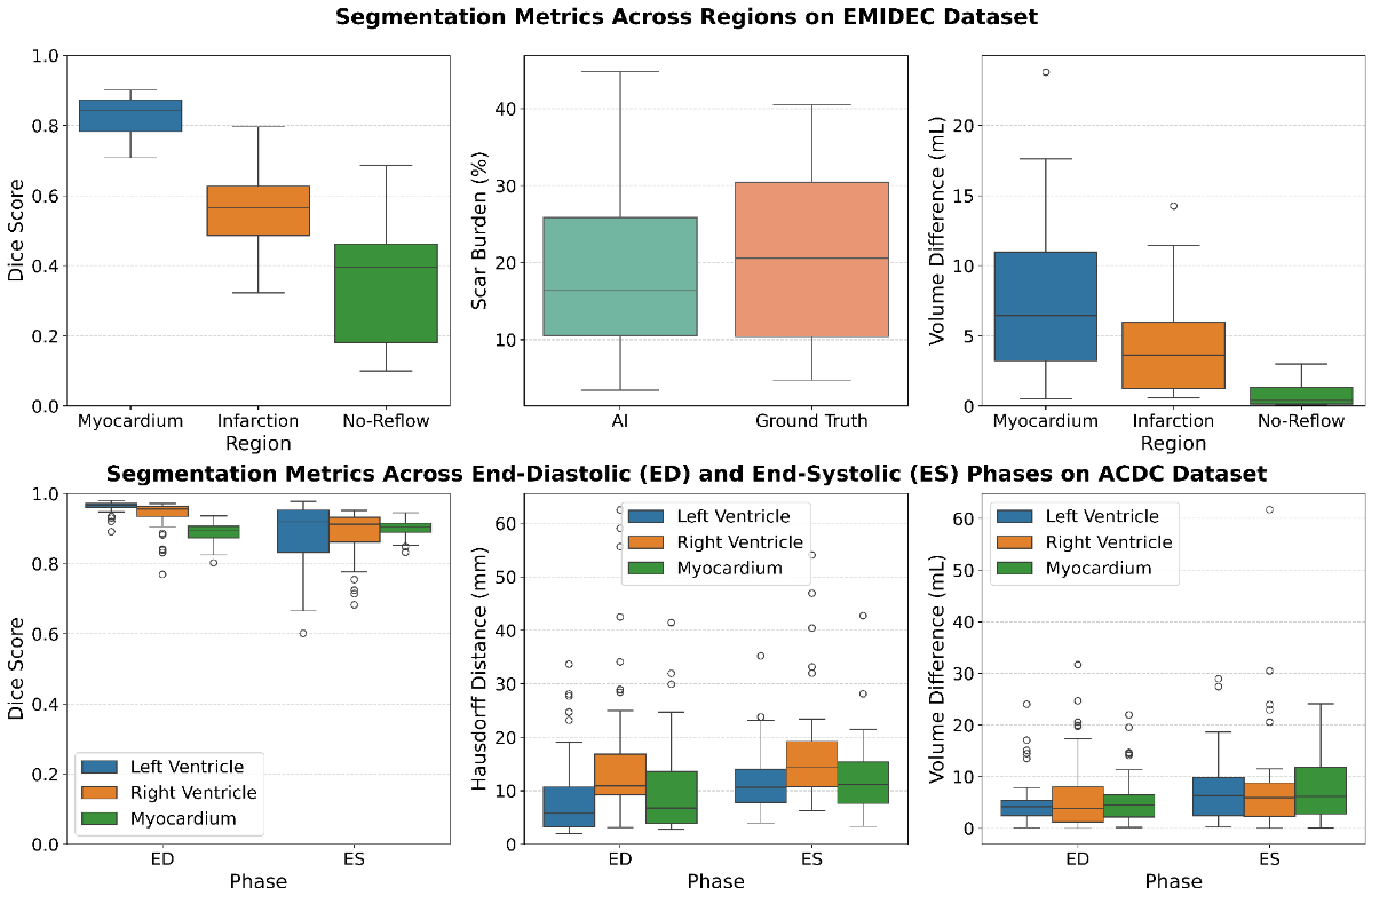
\includegraphics[width=0.9\linewidth]{images/segmentation_metrics.pdf}
    \caption{Quantitative evaluation on the EMIDEC (top) and ACDC (bottom) datasets. Performance is assessed using Dice score, Hausdorff distance (HD), volume difference, and scar burden (\% infarcted myocardium).}
    \label{fig:metrics}
\end{figure}
Figure~\ref{fig:reports} illustrates automatically generated patient reports integrating segmentation results, quantitative biomarkers, and representative MRI slices into a structured clinical summary.
\begin{figure}[!ht]
    \centering
    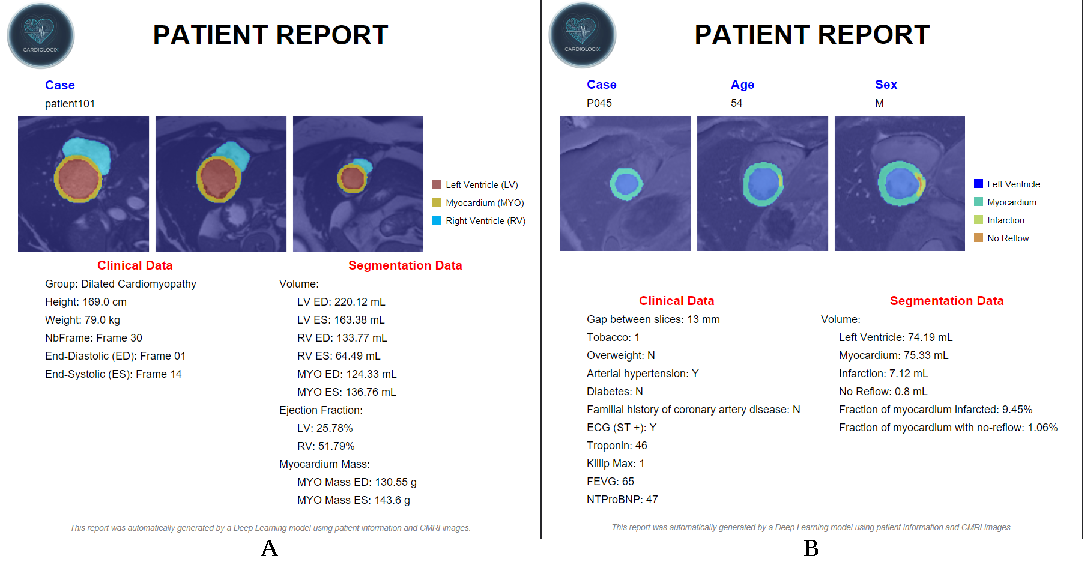
\includegraphics[width=0.9\linewidth]{images/reports.pdf}
    \caption{Examples of patient reports automatically generated with \textit{Myopari}. A) ACDC cine CMR case with dilated cardiomyopathy. B) EMIDEC LGE CMR case with myocardial infarction. Each report includes patient metadata, representative segmented MRI slices, quantitative cardiac measurements, and clinically relevant biomarkers.}
    \label{fig:reports}
\end{figure}
Table~\ref{tab:hardware} summarizes deployment performance on different hardware platforms. Jetson Orin Nano required only 2.4~GB GPU memory and approximately 2.2~s per patient, while Raspberry Pi~5 completed inference in approximately 10.6~s using CPU-only computation. No statistically significant differences in segmentation performance were observed across devices ($p>0.05$).
\begin{table}[!ht]
\centering
\caption{Comparison of inference performance across different hardware platforms. Average inference time, GPU memory usage, energy consumption, and hardware cost are reported for CMR segmentation on the EMIDEC and ACDC datasets. No statistically significant differences in segmentation performance were observed across devices (p>0.05).}
\label{tab:hardware}
\begin{tabular}{lccccc}
\toprule
\multirow{2}{*}{\textbf{Devices}} &
\multicolumn{2}{c}{\textbf{Time (s/patient)}} &
\textbf{GPU Memory} &
\textbf{Energy} &
\textbf{Cost} \\
\cmidrule(lr){2-3}
& \textbf{EMIDEC} & \textbf{ACDC} & \textbf{(GB)} & \textbf{(J/image)} & \textbf{(USD)} \\
\midrule
RTX 4070 SUPER & 1.1 & 1.3 & 5.5 & 30.2 & $\sim$1300 \\
Jetson Orin Nano              & 1.3 & 2.2 & 2.4 & 15.3 & $\sim$250 \\
Raspberry Pi 5                & 7.4 & 10.6 & --  & 8.9  & $\sim$70 \\
\bottomrule
\end{tabular}
\end{table}


\section{Impact in Resource-Constrained Settings (RCS)}

\textit{Myopari} addresses several barriers to AI-assisted CMR analysis in resource-constrained healthcare settings. By enabling inference on affordable edge devices such as the NVIDIA Jetson Orin Nano and Raspberry Pi 5, the system substantially reduces hardware cost and energy consumption compared with conventional GPU workstations, making deployment feasible for healthcare providers with limited computational infrastructure.

The Napari-based GUI enables automated segmentation, quantitative analysis, 3D visualization, and structured report generation through a simple point-and-click workflow, without requiring programming expertise. It also supports (optional) interactive review and correction of AI-generated contours, enabling a human-in-the-loop workflow with expert oversight (when available).

The low deployment cost allows multiple edge devices to be distributed across departments or clinical sites instead of relying on a single GPU workstation, improving scalability and accessibility. Combined with automated quantitative reporting, this can reduce reporting time and support non-specialist clinicians and healthcare providers, where cardiac imaging expertise is limited. Furthermore, \textit{Myopari} is fully open-source, promoting reproducibility, sustainability, and wider adoption of AI-assisted CMR analysis in LMICs. The framework can also be extended to other MRI sequences and more widely available imaging modalities, such as X-ray computed tomography and ultrasound. 

\section{Discussion \& Conclusion}

This study demonstrates that accurate CMR segmentation can be achieved using lightweight models deployed on low-cost edge devices without compromising segmentation performance. The proposed \textit{Myopari} FC-DenseNet retains the dense connectivity and segmentation robustness of the original FC-DenseNet architecture while reducing the model size from 9.4 million to only 1.4 million parameters ($\approx 7\times$ reduction). This reduction is achieved through a shallower network architecture with fewer dense blocks and fewer layers per block, enabling fast and accurate inference on low-cost edge devices. By integrating segmentation, quantitative analysis, visualization, and automated reporting into a single Napari plugin, \textit{Myopari} provides a practical software solution that extends beyond model inference. Optional interactive contour editing further enables a human-in-the-loop workflow for quality assurance when CMR expertise is available. \textit{Myopari} can also be combined with large language models (LLMs) to generate clinically interpretable narrative reports, as demonstrated in this \href{https://github.com/QBioImaging/myopari/blob/main/reports/myopari_report_patient101_4d.nii.md}{example patient report}.

This study has several limitations. Validation was performed on two single-vendor public datasets, and additional evaluation on multi-center and multi-vendor datasets is needed. In addition, the LLM-generated narrative reports have not yet been clinically validated and require systematic evaluation and expert oversight to ensure their accuracy and reliability.

In summary, our proposed lightweight AI-driven CMR analysis runs efficiently on portable, low-cost, energy-efficient devices, allowing both specialist and non-specialist clinicians in under-resourced settings to easily generate accurate quantitative cardiac reports, expand diagnostic access, and ultimately improve patient outcomes.

\subsubsection{Acknowledgements} 
This study received funding from the FCT--Portuguese Foundation for Science and Technology through grants
UID/04326/2025, \linebreak
UID/PRR/04326/2025,
LA/P/0101/2020
(\url{https://doi.org/10.54499/LA/P/0101/2020}),
2025.02647.BDANA
(\url{https://doi.org/10.54499/2025.02647.BDANA}),
`la Caixa' Foundation and FCT, I.P.\ under project 
LCF/PR/HR22/00533,
NVIDIA GPU Hardware Grant,
and EU Horizon Europe project IMAGINE, GA No.~101094250 (\url{https://doi.org/10.3030/101094250}).
\section*{Disclosure of Interests}
The authors declare no competing interests.


\bibliographystyle{splncs04}
\bibliography{paper}

\end{document}
